\def\year{2015}
\documentclass[letterpaper]{article}
\usepackage{aaai}
\usepackage{times}
\usepackage{helvet}
\usepackage{courier}
\usepackage{graphicx}
\usepackage{amsfonts}
\frenchspacing
\setlength{\pdfpagewidth}{8.5in}
\setlength{\pdfpageheight}{11in}
\pdfinfo{
/Title (Insert Your Title Here)
/Author (Put All Your Authors Here, Separated by Commas)}
\setcounter{secnumdepth}{0}
\begin{document}
%
\title{Gaussian Processes for Modelling of Crowds}
\author{CS4246 Project: Planning and Decision Making in the Real World  \\ \\
{\bf Team 04} \\
Huang Wei Ling, A0101200R\\
Nathan Azaria, \\
Ng Hui Xian Lynnette, A0119646X\\
Nguyen Duc Thien, A0093587M\\
Oh Shunhao, A0065475X\\
}
\maketitle
\begin{abstract}
\begin{quote}
Crowd management is essential in events where the committee has to plan and organize in an effective and efficient manner, taking into consideration factors such as the facility, size and demeanor of the crowd and crowd control. The motion analysis of crowd in multivariate timeseries data requires an effective model to represent the data. In this report, we illustrate the use of Gaussian Processes to model crowd distributions from noisy and unevenly-sampled position data, and we explore how this representation can be used to predict the density of the population for future data.
\end{quote}
\end{abstract}

\section{1.  Introduction}
In this report, we propose the use of Gaussian process(GP) for modelling of crowds. Particularly, we will discuss how we exploit the desirable properties of Gaussian process(GP) model, some of the advantages that the model provide, the critical requirements of our proposed application as well as how people can make use of the results of our analysis to plan and make decisions for future crowd controlling or crowd management. Next, we will touch on the technical details which includes the fitting on the characteristics of Gaussian process(GP) model for the application, additional findings we gathered and modification of the model to enhance performance. The third section of the report will be a detailed experimental plan we will be using to perform and evaluate the performance of Gaussian process(GP) for modelling of crowds. Lastly, the report will end with an interesting factor we will be exploring in this project.

\section{2.  Gaussian Process Regression for Motion Analysis of Crowds}

We define a position of a person as a discrete vector sequence in $\mathbb{R}^3$. Let $z \epsilon \mathbb{R}^3$ be the position ($x, y, z$), where x corresponds to a point of time, y as the function of the coordinates and z as the axis. We consider a position sequence $z_n = {x_i, y_i, z_i} | i = 1,...,n$. \\

{\bf2.1  Constructing Mean and Covariance Functions} \\

Gaussian process regression model is represented as $y = f($x$) + \epsilon$, which $y$ is a dependent variable expressed in terms of an independent variable x through a function $f($x$)$ with a noise term $\epsilon \sim N(0, \sigma^2)$. The function $f$ can be interpreted as a probability distribution over functions, \\

$ y = f(x) \sim GP(m(x), k(x,x^\prime))$ \\

where $m(x)$ is the mean function of the distribution and $k$ is a covariance function which describes the relationship between two values of the independent variable, $x$ and $x^\prime$, as a function of the kernel distance between them. \\

In our project, we are using a heteroscedastic model that works the same way as a Gaussian Process(GP) model. However, this model allows the use of different variances for the noise terms of the observations, $\epsilon_i \sim N(0, \sigma_i^2)$, giving different weights to each observation. Therefore, it serves to fit observations with smaller noise and choose to ignore those with larger noise. \\

By experimenting with different kernel functions, we obtain the final GP model using a linear combination of a Multilayer Perceptron (MLP) and a constant Bias as kernel function as they consistently output acceptable results for regressions on our datasets. MLP, also known as arc sine kernel or neural network kernel, can be optimized to represent a complex non-linear function. \\

{\bf2.2  Qualitative Advantages} \\

There are many advantages to using the Gaussian Process model. One key property of the data is that it is unevenly sampled, with multiple large gaps in between the position readings $(x,y,z)$ of each individual. As these points are discrete and finite, the crowd densities at certain positions and times are not represented by the data. After processing the data with using the Gaussian Process model, we will be able to fill in these gaps in data. \\

Another benefit is that the Gaussian Process model provides both the mean and variances of the position of the user at each point of time, allowing us to construct a probability distribution of the user's position at each point of time. A probability distribution allows us to compute the proportion of the crowd at any point of time, over any defined region. \\

One reason why this model is a good fit is because of the correlation between the current position of each individual and the future positions. Thus the coordinates of the individuals each modelled as a trajectory over time. There have been past usages of the GP model trajectory prediction in data. For example, in a paper by {\it Marco A. F. Pimentel, David A. Clifton, Lionel Tarassenko}, Gaussian Processes were used to model the trajectory of human vital signs. \\

%-COMMENT OUT-
% On the other hand, we propose Gaussian process(GP) model as it can specify the variance of noise at each point, deal with gaps between data if there is a break in between the event or for events which last a few days. Importantly, the prediction is probabilistic (Gaussian) so that one can compute the empirical confidence intervals and exceedance probabilities that might be used to refit the prediction for future crowd controlling of events. \\
%-COMMENTED OUT-

Gaussian process model fits our application well as we can can specify the variance of noise at each point, given any regions and we are able to predict the output by integrating over the regions, whereas for other curve fitting methods, the variances are unknown to us and therefore we cannot integrate over the regions we are interested to find the population density.


{\bf2.3  Important Requirements} \\

Some of the important requirements of the proposed application of crowd modelling include the use of big data and the data of different demographics of approximately 1224 users and locations of 2 levels in the building. \\

{\bf2.4  Interpreting  Outputs} \\

In our project experiment, we will be selecting 50 random time intervals, plot a multivariate distribution at each of these 50 time intervals and integrate it. The sum of all the 50 integrated intervals will show the expected amount of people there are at each point of time. The outputs of the Gaussian Process(GP) model are useful in helping human users or experts in using a sample of people in the data to predict the population density of a particular area at any instance of time.

\section{3.  Technical Approach}

{\bf3.1  How does the GP model you’re using fit the requirements of your proposed application exactly?} \\

input of 3 graphs \\

{\bf3.2  Additional Insights} \\

An issue with $x$, $y$ and $z$ coordinates is that they may not be a very good model of crowd densities, especially for less open spaces. 
In our dataset, because the event is a conference, the spaces are wide open, this is not an issue as individuals with close together $x$, $y$ and $z$ coordinates are likely to be close to each other as well. However, in buildings with narrower corridors and tighter spaces, individuals with similar $x$, $y$ and $z$ coordinates may actually be very far apart from each other. Figures XXX and XXX illustrate this idea.

\begin{figure}[h!]
  \centering
    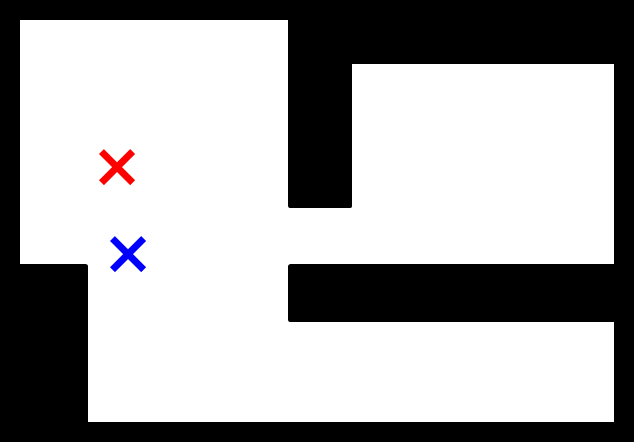
\includegraphics[width=150px,natwidth=634,natheight=442]{openspace1.png}
  \caption{Points with similar $x$ and $y$ coordinates in an open space}
\end{figure}

\begin{figure}[h!]
  \centering
    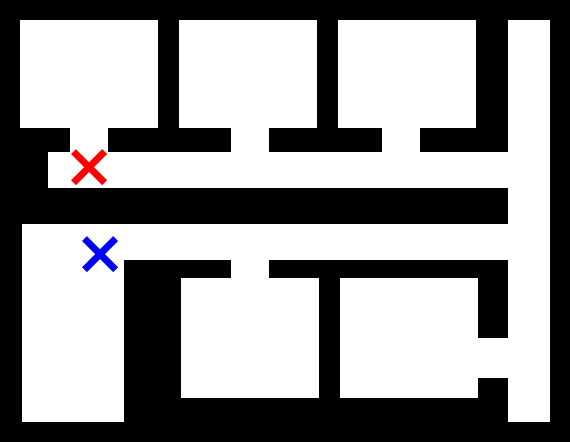
\includegraphics[width=150px,natwidth=570,natheight=442]{openspace2.png}
  \caption{Points with similar $x$ and $y$ coordinates in a less open space}
\end{figure}

{\bf3.3  Novel Modification} \\

To model less open spaces, we can use an alternative modelling, provided we know the layout of the area. Instead of using the $x$, $y$ and $z$ coordinates of each user, we can use shortest path distances as the attributes instead. We first define a set of reference points at significant points $p_1,p_2,\cdots,p_k$ in the area. For each data point $d$, we compute the shortest paths $s_i$ from the data point to each of the reference points $p_i$. This is shown in Figure XXX. \\

We then use the same Gaussian Process model as before using the values $s_i$ as the attributes. The advantage of using shortest paths as a metric is the geometry of the map has been abstracted out; two points with similar values of $s_i$ must be points that are close to each other. (given enough reference points)\\

\begin{figure}[h!]
  \centering
    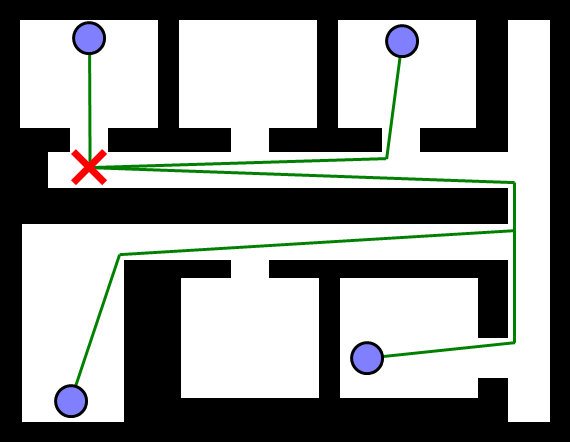
\includegraphics[width=150px,natwidth=570,natheight=442]{shortestpaths.png}
  \caption{The shortest paths from a data point to four reference points}
\end{figure}

However, it is important to note that with this formulation, the reference points must be carefully picked for a good prediction. (spread out, and preferably near the areas you are concerned about)

By knowing the predicted densities of people within a defined radius of a certain point, we can do better crowd control. For example, given a prediction that people tend to crowd around a certain area at a certain point of time, obstacles can be reduced or shifted about. Personnel can also be deployed to facilitate crowd movement. This will be useful in cases of MRT breakdowns. \\

In addition, by being able to predict the crowd density of an area in a future timestamp, we can do a certain form of path prediction. This can help in deciding building maps and object placements. For example, if we can model that generally if the crowd density of the facial shop increases, generally the crowd density of the restrooms will increase in the next timestamp, we might want to consider putting the restrooms in near proximity to the facial shop. Or if we can model that the crowd density streams from one product to another in a supermarket, we might want to consider placing both products near each other so shoppers can easily reach for both products at once, hence increasing the sales revenue.  \\

\section{4.  Experimental Evaluation}

{\bf4.1  Experimental Setup} \\

We prepare and implement our experiments in Python. For the Gaussian Process modeling and regression, we use the library Sheffield GPy with the help of Scipy and Numpy for numerical calculation and representation. We use the data structure and data analysis tools provided by the module Pandas to store, access and analyze our dataset. \\

The Stochastic Variational Inference method using the climin module and AdaDelta rule and direct optimization using BFGS method are used to regress our model. By observing the results from several samples of our dataset, the latter provides more desirable results and is chosen for further experiments. \\

We experimented with several families of kernel functions including the Radial Basis function (RBF), Exponential function, Matern52, Matern32 and Multilayer Perceptron (MLP). The experiments also involve varying their respective parameters such as noise values, relaxing or fixing constraints, changing initial values and inducing points and combining with various White and Bias kernels. Finally, the combination of kernel functions that yield consistent results as observed cross different samples from our dataset is selected to build our GP model for further application. \\

We extract the X, Y and Z coordinates from the GPS location and perform the regression against the timestamps provided in the dataset. We also generate a common set of timestamps to predict the user movements against, in which we generate the mean and variance from the output of the GP we had earlier regressed. \\

Following which, we analyse the crowd density within a certain radius of a point by counting the number of unique tags within the specified radius. \\  

{\bf4.2  Real-World Dataset} \\

We test our approach using a Attendee Meta-Data (AMD) Hope RFID Dateset from which data is collected from 1224 hackers attending The Last HOPE Conference from 18-20 July 2008, located in Hotel Pennsylvania, New York City. The data set details descriptions of their interests, interactions through instant messages, and location over the course of the conference. \\

{\bf4.3  Are there more than one type of GP model/variant that can be used in your proposed application? Can other types of linear or non-linear regression models be used? If so, how do you plan to empirically compare their performance? What quantitative/ empirical advantages (and/or limitations) do the GP model or its variant offer over the other evaluated models?} \\

Several types of GP models were experimented with, including Stochastic Variance Gaussian Processes and Sparse Gaussian Processes. We also performed experiments with all the different types of kernels provided by the GPy library, including linear kernel and white kernel. We also tweaked the input parameters, such as the variance of the kernels to experiment with the data. The GP model-variant that we proposed has the co-variance matrix and mean that fits the data the best. \\ 

A linear regression model will not suit the data as there is little correlation between the points; the GPS coordinates change randomly with respect to the timestamp as users move randomly within the conference area. The advantage the GP model in the application is its use of all the samples and feature information to perform the prediction, while allowing for the training data to have different or uneven sampling rates. In our case, not all the users have their GPS signals sampled at the same timestamps, nor do they all have the same number of sample points. We have only a few dimensions, so we are not affected by the property where GP loses its computational efficiency in high dimensional spaces -- on average, each GP model takes less than a minute to compute; the longest a model has taken is 3 minutes. The prediction is probabilistic so we can compute empirical confidence levels that may be useful in our prediction of crowd density. In addition, the use of a GP model allows the detection of incomplete paths, i.e. loss of GPS signals, resulting in no data for certain time periods. It enables the comparison of noisy data, which is evident in the case of GPS signals and random user movements.
\\

Note: Can run the kernels that failed and put plots if needed (i.e. not enough images)

\section{5.  Wow factor}

\section{6.  Conclusion and Contribution}

\section{7.  References}

\end{document}
